\chapter{User manual}


   \begin{center}
    \vspace*{3\baselineskip}
    \large
    \bfseries
    XOXOmail\\[2\baselineskip]
    
    User Manual \\
    \normalfont
    \large
    
    	
    
\includegraphics[height=18em]{login_screen}
  \end{center}

\newpage

\section*{Contents}
\begin{enumerate}
\item{}Logging in
\item{}Viewing the inbox
\item{}Sending a message
\item{}Instant messages
\item{}Flash and Override messages
\item{}Configuring the settings
\end{enumerate}


\newpage
\section*{Logging in}

After starting the XOXOmail application you will be prompted with a login screen. In order to login, simply press the login button below the password field. There is no need to enter any information in the Email and Password field as this has not yet been implemented. 

  \begin{center}
    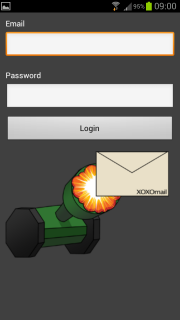
\includegraphics{logingui1}
  \end{center}
  \newpage
  
\section*{Viewing the inbox}
To view the inbox, make sure the inbox tab i selected. You will then see a list of all messages currently in the inbox. If you want to sort these messages, simply press the sort button indicated in the screenshot below.   

  \begin{center}
    \includegraphics{viewinboxarrows}
  \end{center}
\newpage
You can then select the desired sorting algorithm by pressing the different options presented. 
  \begin{center}
    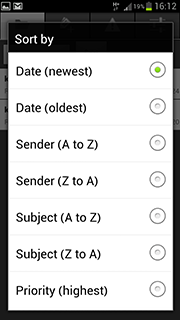
\includegraphics{SortBy}
  \end{center}

\newpage
If you want to view any of the messages currently in the inbox, you can press the messages displayed on the screen. You will then be brought to the message view. 
\newline 
\newline 
From the message view you can see the sender of the message, the message attributes and the actual message text. You also have the opportunity to change between received messages, reply to a message and forward the received message. This is done by pressing the respective buttons at the bottom of the screen.

  \begin{center}
    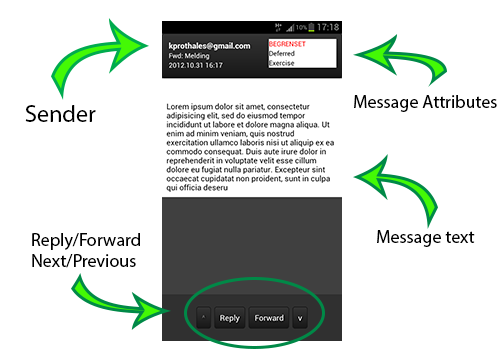
\includegraphics{ViewMessageArrows}
  \end{center}

\newpage
\section*{Sending a message}
To send a new message, you must first make sure you have the send message tab selected. You will then be presented with the send message view. \newline \newline First you must select the recipient of the message to be sent. This can be done by either typing in the recipient manually or pressing the contacts button.  
  \begin{center}
    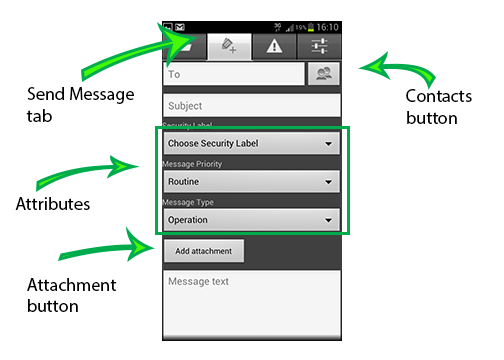
\includegraphics{sendmessagearrows}
  \end{center}
  \newpage
  If the contacts button is pressed, a new window will open displaying your contacts. Pressing one of these contacts will add the address to the "To" field.
  \begin{center}
    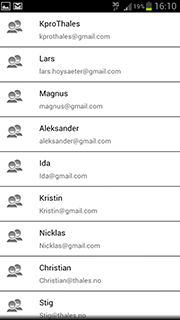
\includegraphics{Contacts1}
  \end{center}
\newpage
After choosing a recipient you must add a subject to your message. This is done by typing in the subject in the field below the recipient field.
\newline 
\newline 
The next step is to select which attributes your message will include. You will need to select the label, priority and type of the message, if the attributes are not selected, the default values will be added to the message. 

\begin{figure}[h]
\makebox[\textwidth]{%
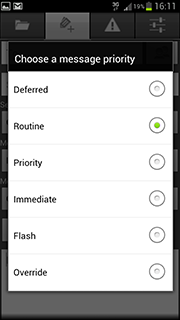
\includegraphics[width=0.30\textwidth]{ChooseMessagePriority}%
\hfill    
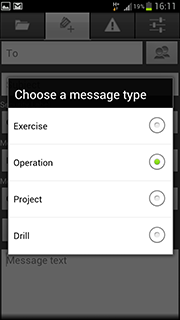
\includegraphics[width=0.30\textwidth]{ChooseMessageType}%
\hfill    
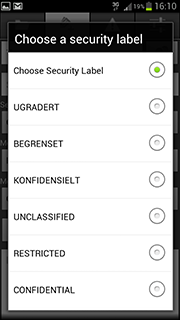
\includegraphics[width=0.30\textwidth]{ChooseSecurityLabelz}%
}%
\caption{Choosing attributes}
\label{fig:OlimpicCircleTT1}
\end{figure}

\newpage
After adding the message attributes you have the opportunity to add an attachment to your message. This can be an image from the camera, an image already stored on the phone or your current GPS location. 

 \begin{center}
    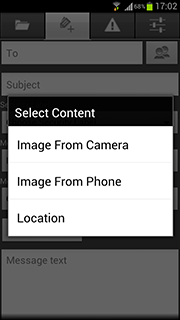
\includegraphics{attachments}
  \end{center}

Finally the actual message text can be added to the message. This is done by pressing the Message text field and typing in the desired text. To send your message, simply press the send button at the bottom of the screen. 
\newpage
\subsubsection{Instant messages}
To send an instant message, you must have the instant message tab selected. The instant message view shows you the predefined recipient and attributes. The predefined values are set in the settings menu. To send an instant message you simply type in the message text and press the send button. 
 \begin{center}
    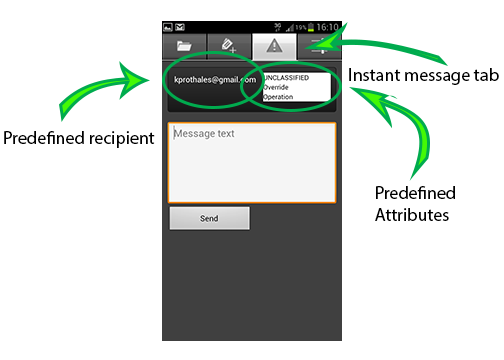
\includegraphics{instantmessagearrows}
  \end{center}


\newpage
\section*{Flash and Override messages}




When receiving a message with message priority set to Flash or Override, a red popup will cover your screen. You can then view this message, or press cancel to close the window.

 \begin{center}
    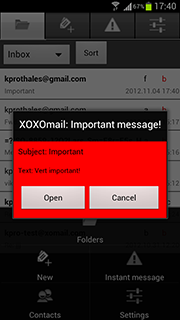
\includegraphics{FLASH}
  \end{center}


\newpage
\section*{Configuring the settings}

To alter the various settings in the application, you must have the settings tab selected.
 \begin{center}
    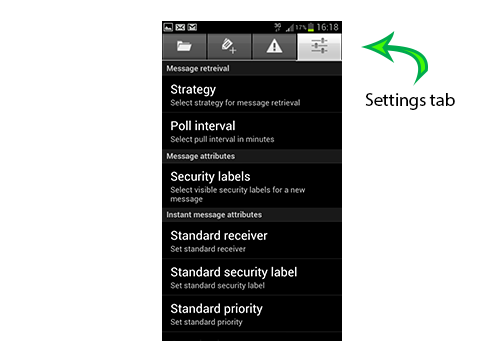
\includegraphics{settingsarrow}
  \end{center}

In the settings tab you have 4 different categories of configurable settings:
\begin{itemize}
\item{}Message retrieval
\item{}Message attributes
\item{}Instant message attributes
\item{}Location data
\end{itemize}

\newpage
In the message retrieval section you have the ability to choose the message retrieval strategy and poll interval. 
\newline 
\newline
There are 2 message retrieval strategies available at this time: push and pull. When pull is selected, the messages in the inbox are loaded every given interval. The application queries the server for new messages after a set interval has passed. \newline 
If push is selected the application will load all the messages in the inbox after startup. When a new message arrives the server will push the message to the application and display it in the inbox. 

\begin{figure}[h]
\makebox[\textwidth]{%
\hfill  
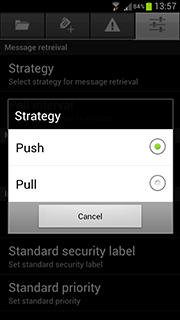
\includegraphics[width=0.40\textwidth]{PullStrategy}%
\hfill    
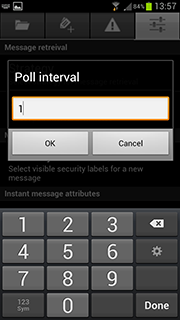
\includegraphics[width=0.40\textwidth]{PollInterval}%
\hfill    

}%
\caption{Pull strategy and poll interval}
\label{fig:OlimpicCircleTT1}
\end{figure}
 
\newpage
In the message attributes section you have the ability to select which attributes that you would like to choose amongst when sending a message.
   \begin{center}
    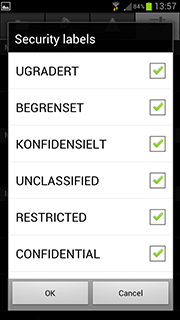
\includegraphics{SecurityLabelsShown}
  \end{center}
\newpage
In the instant message attributes section you have the ability to set the different standard values for sending an instant message. These include:

\begin{itemize}
\item{}Standard receiver
\item{}Standard security label
\item{}Standard priority
\item{}Standard type
\end{itemize}

\begin{figure}[h]
\makebox[\textwidth]{%
\hfill  
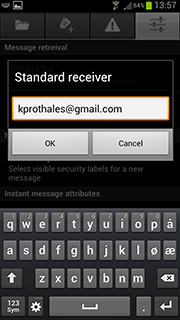
\includegraphics[width=0.24\textwidth]{StandardReceiver}%
\hfill    
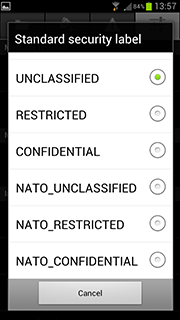
\includegraphics[width=0.24\textwidth]{StandardSecurityLabel}%
\hfill    
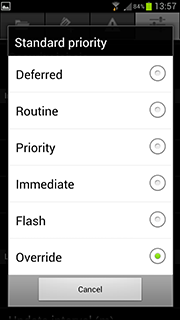
\includegraphics[width=0.24\textwidth]{StandardPriority}%
\hfill    
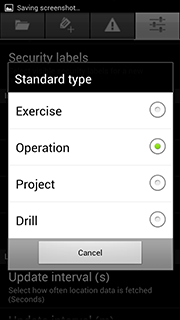
\includegraphics[width=0.24\textwidth]{StandardType}%
\hfill   
}%
\caption{Instant message standard values}
\label{fig:OlimpicCircleTT1}
\end{figure}

\newpage
In the location data section you can choose when the gps position is fetched. This is done by setting how often it should try to update the gps position in seconds, and also how far you need to travel in order update the gps coordinates. 

\begin{figure}[h]
\makebox[\textwidth]{%
\hfill  
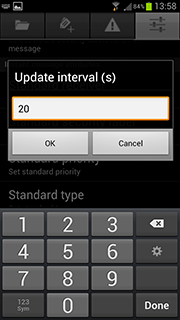
\includegraphics[width=0.49\textwidth]{GPSUpdateInterval}%
\hfill    
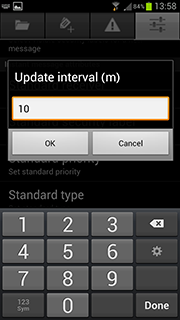
\includegraphics[width=0.49\textwidth]{GPSUpdateIntervalMeters}%
\hfill    

}%
\caption{GPS settings}
\label{fig:OlimpicCircleTT1}
\end{figure}

